\documentclass[12pt, a4paper]{book}%, oneside
\setcounter{secnumdepth}{3}
\setcounter{tocdepth}{3}
\usepackage[headings]{fullpage}
\usepackage{setspace}
\usepackage{titlesec}


%setcounter{secnumdepth}{4}

\titleformat{\paragraph}
{\normalfont\normalsize\bfseries}{\theparagraph}{1em}{}
\titlespacing*{\paragraph}
{0pt}{3.25ex plus 1ex minus .2ex}{1.5ex plus .2ex}
\usepackage{graphicx}
\usepackage{float}
\usepackage{subfig}
\usepackage{lipsum}
\usepackage{enumitem}
\usepackage{array}
% \usepackage{xtab}
\usepackage{multirow}
\usepackage{booktabs}
\usepackage{appendix}
\usepackage[pdfborder={0 0 0}, colorlinks=true, linkcolor=black, citecolor=blue]{hyperref}
\usepackage[printonlyused]{acronym}
\usepackage{algorithmic}
\usepackage{algorithm}
\usepackage{ifpdf}
\usepackage{graphicx}
\usepackage{float}
\usepackage{subfig}
\usepackage{array}
% \usepackage{xtab}
\usepackage{multirow}
\usepackage{booktabs}
\usepackage{appendix}
\usepackage[pdfborder={0 00},colorlinks=true,linkcolor=black,citecolor=blue]

\usepackage{amsmath}
\usepackage{bm}
\usepackage[table]{xcolor}
\usepackage{tikz,calc}
\usetikzlibrary{positioning}
\usetikzlibrary{shapes}
\usepackage{listings}
\usepackage{color}
\definecolor{lightgray}{rgb}{.9,.9,.9}
\definecolor{darkgray}{rgb}{.4,.4,.4}
\definecolor{purple}{rgb}{0.65, 0.12, 0.82}
% \setlength{\parindent}{0pt}
\usepackage[utf8]{inputenc}
\usepackage[english]{babel}
\usepackage[utf8]{inputenc}
\usepackage{xcolor}
\usepackage{minted}

\parindent=0pt
\definecolor{RoyalBlue}{cmyk}{1, 0.50, 0, 0}

\lstset{language=C++,
    keywordstyle=\color{RoyalBlue},
    basicstyle=\ttfamily\bfseries\scriptsize\ttfamily,
    commentstyle=\texttt\texttt\color{gray},
    stringstyle=\bfseries\bfseries\ttfamily,	
    showstringspaces=false,
    breaklines=true,
    frameround=ffff,
    frame=single,
    rulecolor=\color{black},
    xleftmargin=\dimexpr\fboxsep-\fboxrule,
    xrightmargin=\dimexpr\fboxsep-\fboxrule,
    gobble=8
}

\newcommand{\submissionDay}{15}
\newcommand{\submissionMonth}{December}

\newcommand{\submissionYear}{2019}
\newcommand{\submissionDate}{\submissionDay~\submissionMonth~\submissionYear}
\newcommand{\typeOfThesis}{Semester Project}

\newcommand{\titleOfThesisOne}{Semester Project and Explanation of Source Codes related to some problems}

\newcommand{\authorOfThesis}{Amir Haytham Salama}
\newcommand{\supervisorOne}{Prof. Dr. Ahmad Fouad}

\newcommand{\includefig}[4]{
    \begin{figure}[ht]
     \centering
      \includegraphics[width=#1\textwidth]{images/#2}
      \caption{#3}
      \label{#4}
    \end{figure}
}

\newcommand{\includefigWSC}[5]{
    \begin{figure}[ht]
     \centering
      \includegraphics[width=#1\textwidth]{images/#2}
      \caption[#3]{#4}
      \label{#5}
    \end{figure}
}

\newcommand{\includeeps}[4]{
\includefig{#1}{#2.eps}{#3}{#4}
}

\newcommand{\includeepsWSC}[5]{
\includefigWSC{#1}{#2.eps}{#3}{#4}{#5}
}


\ifpdf
\pdfinfo {
	/Author (\authorOfThesis)
	/Title (\titleOfThesisOne)
	/Subject (\typeOfThesis)
	/Keywords ()
	/CreationDate (D:20090707085533)
}
\fi

\begin{document}
% \overfullrule=5pt
\pagestyle{plain}
\pagenumbering{Roman}

\newcommand{\titlePage}{

%
\hfill
%
\begin{center}
	\vspace{2cm}
	\doublespacing
	{\Huge \textbf{\titleOfThesisOne}}\\
	\singlespacing
	\vspace{2cm}
	{\large \textbf{\typeOfThesis}}\\
	
	\vfill
	\parbox{1cm}{
  		\begin{large}
    			\begin{tabbing}
       			Author: \hspace{2cm}  
        			\=\authorOfThesis\\[2mm]
      			Supervisors: 
        			\>\supervisorOne\\[2mm]
				\>\supervisorTwo\\[2mm]
				\>\supervisorThree\\[2mm]
      			Submission Date: 
        			\>\submissionDate\\
    			\end{tabbing}
  		\end{large}
	}\\
\end{center}
\clearpage
}
%++++++++++++++++++++++++++++++++++++++++++++++++++++++++++++++++++++
%\titlePage
%\thispagestyle{empty}\ \clearpagehttps://www.overleaf.com/project/5de74e793bbb9a00017e0825
\titlePage
%++++++++++++++++++++++++++++++++++++++++++++++++++++++++++++++++++++
\thispagestyle{empty}
This is to certify that:
\begin{itemize}
\item[(i)] the documentation comprises only my original work
\item[(ii)] due acknowledgement has been made in the text to all other material used
\end{itemize}

\vspace{2cm}
\begin{flushright}
\rule[0mm]{6cm}{0.2mm}\\
\authorOfThesis\\
\submissionDay~\submissionMonth,~\submissionYear\\
\end{flushright}
\clearpage


\chapter*{Acknowledgments}
\addcontentsline{toc}{chapter}{Acknowledgments}
\label{chap:ack}
After thanking Allah (SWT), I would like thank Prof. Dr. Ahmad Fouad for accepting me to work on his project and his effort with in the semester. I would like also to thank him for introducing my project of our course Analysis and Design of Algorithms (CS312) and helping me getting through a lot of difficulties throughout the semester.

\chapter*{Abstract}
% \addcontentsline{toc}{chapter}{Abstract}
\label{chap:abstract}
In this work, I am going to exaplain some of our algorithm course and some of our tutrials codes. Also, i describe the algorithms in detailed and at the end there is a project explaining the object who wants to find the shortest path using BFS algorithm. I show different test cases for some algorithms, to make much more doable.
\addcontentsline{toc}{chapter}{Contents}
\tableofcontents

\clearpage 

\pagestyle{headings}
\pagenumbering{arabic}

% \setlength\parskip{15pt}
\setlength\parskip{.5\baselineskip plus .2\baselineskip
	minus .4\baselineskip}
% \setlength\parskip{.5\baselineskip \@plus .1\baselineskip \@minus ..1\baselineskip}


\chapter{Sorting Algorithms}

\section{Counting Sort $o(n)$}
\textbf{{\Large{Problem Description}}}

Given an (unsorted) array of n elements, can we sort them in $O(n)$ time?\newline
    
\textbf{{\Large{Solution}}}\newline\newline
\textbf{{\large{Sorting in Linear Time (Counting Sort)}}}\newline\newline
If the array $A$ contains n integers with small range \textbf{$[L .. R]$}, we can use the Counting Sort algorithm. For the explanation
below, assume that array $A$ is \textbf{{2, 5, 2, 2, 3, 3}}. The idea of Counting Sort is as follows:

1. Prepare a \textbf{‘frequency array’ $f$} with size $k$ = $R-L+1$ and initialize $f$ with zeroes.
On the example array above, we have $L$ = 2, $R$ = 5, and $k$ $=$ 4.
\newline
\\
2. We do one pass through array A and update the frequency of each integer that we see,
i.e. for each i ∈ $[0..n-1]$, we do \textbf{$f[A[i]-L]++$}.
On the example array above, we have \textbf{$f[0] = 3, f[1] = 2, f[2] = 0, f[3] = 1$}.
\newline
\\
3. Once we know the frequency of each integers in that small range,
we compute the prefix sums of each i, i.e. \textbf{$f[i] = [f-1] + f[i] ∀i ∈ [1..k-1]$}.
Now, f[i] contains the number of elements less than or equal to i.
On the example array above, we have \textbf{$f[0] = 3, f[1] = 5, f[2] = 5, f[3] = 6.$}
\newline
\\

4. Next, go backwards from $i = n - 1$ down to $i = 0$.
We place \textbf{$A[i]$} at index $f[A[i]-L] - 1$ as it is the correct location for \textbf{$A[i]$}. We decrement \textbf{$f[ A[i] - L]$} by one so that the next copy of \textbf{$A[i]$}—if any—will be placed right before the current \textbf{$A[i]$}. On the example array above, we first put $A[5]$ = 3 in index \textbf{$f[A[5] - 2] - 1 = f[1] - 1 = 5 - 1 = 4$} and decrement \textbf{$f[1]$ to 4}. Next, we put \textbf{$A[4] = 3$} —the same value as \textbf{$A[5] = 3$}—now in index \textbf{$f[A[4] - 2] - 1 = f[1] - 1 = 4 - 1 = 3$} and decrement $f[1]$ to $3$. Then, we put \textbf{$A[3] = 2$} in index \textbf{$[A[3] - 2] - 1 = 2$} and decrement \textbf{$f[0]$ to $2$}. We repeat the next three steps until we obtain a sorted array: \textbf{{2, 2, 2, 3, 3, 5}}. The time complexity of Counting Sort is $O(n+k)$.
\newline
\\
\textbf{{\Large{Implementation}}}

\begin{lstlisting}{c++}
        #include <bits/stdc++.h>
        
        using namespace std;
        int noOfElements;
        
        void countingSort(vector<int> &v){
            int max_ele = *max_element(v.begin(), v.end());
            vector<int> count_(max_ele + 1, 0);
            for(int i = 0; i < (int)v.size(); ++i)count_[ v[i] ]++;
            for(int i = 1; i <= max_ele; ++i)count_[ i ] += count_[ i - 1 ];
        
            vector<int> new_array( (int)v.size() );
            for(int i = 0; i < (int)v.size(
                                           ); ++i){
                new_array[ count_[ v[i] ]  - 1 ] = v[i];
                count_[ v[i] ]--;
            }
            for(int i = 0; i < (int)v.size(); ++i){
                cout << new_array[i] << " ";
            }
        
        }
        int main(){
            cin >> noOfElements;
            vector<int> v(noOfElements);
            for(int i = 0; i < noOfElements; ++i)cin >> v[i];
            countingSort(v);
        }
\end{lstlisting}

\newpage

\section{Bubble Sort $o(n^2)$} 
\textbf{{\Large{Description}}}

Bubble Sort is the simplest sorting algorithm that works by repeatedly swapping the adjacent elements if they are in wrong order.\newline
    
\textbf{{\Large{Solution}}}\newline\newline
\textbf{{\large{Example:}}}\newline\footnotetext{\url{https://www.geeksforgeeks.org/bubble-sort/}}

1. \textbf{First Pass:}\newline
( \textbf{5 1} 4 2 8 ) –$>$ ( \textbf{1 5} 4 2 8 ), Here, algorithm compares the first two elements, and swaps since 5 $>$ 1.\newline
( 1 \textbf{5 4} 2 8 ) –$>$  ( 1 \textbf{4 5} 2 8 ), Swap since 5 $>$ 4\newline
( 1 4 \textbf{5 2} 8 ) –$>$  ( 1 4\textbf{ 2 5} 8 ), Swap since 5 $>$ 2\newline
( 1 4 2 \textbf{5 8} ) –$>$ ( 1 4 2 \textbf{5 8} ), Now, since these elements are already in order (8 $>$ 5), algorithm does not swap them.
\newline
\\
2. \textbf{Second Pass:}\newline
( \textbf{1 4} 2 5 8 ) –$>$ ( \textbf{1 4} 2 5 8 )\newline
( 1 \textbf{4 2} 5 8 ) –$>$ ( 1 \textbf{2 4} 5 8 ), Swap since 4 $>$ 2\newline
( 1 2 \textbf{4 5} 8 ) –$>$ ( 1 2 \textbf{4 5} 8 )\newline
( 1 2 4 \textbf{5 8} ) –$>$  ( 1 2 4 \textbf{5 8} )\newline
Now, the array is already sorted, but our algorithm does not know if it is completed. The algorithm needs one whole pass without any swap to know it is sorted.
\newline
\\
3. \textbf{Finally}\newline
( \textbf{1 2} 4 5 8 ) –$>$ ( \textbf{1 2} 4 5 8 )\newline
( 1 \textbf{2 4} 5 8 ) –$>$ ( 1 \textbf{2 4} 5 8 )\newline
( 1 2 \textbf{4 5} 8 ) –$>$ ( 1 2 \textbf{4 5} 8 )\newline
( 1 2 4 \textbf{5 8} ) –$>$ ( 1 2 4 \textbf{5 8} )\newline

\newline
\\
\newpage
\textbf{{\Large{Implementation}}}

\begin{lstlisting}{c++}
        #include <bits/stdc++.h>
        
        using namespace std;
        
        int n;
        void bubbleSort(vector<int> &arr){
        	for (int i = 0; i < n-1; ++i)
                for (int j = 0; j < n-i-1; j++)
                    if (arr[j] > arr[j+1])
                        swap(arr[j], arr[j+1]);
        
        }
        
        int main() {
            
        	cin >> n;
        	vector<int> arr(n);
        	for (int i = 0; i < n; ++i)cin >> arr[i];
        	bubbleSort(arr);
        	cout<<"Sorted array: \n";
        	///Print the array after sorting
        	for (int i = 0; i < n; ++i)cout << arr[i] << " ";
        	return 0;
        }
\end{lstlisting}
\newline\newline\newline
\\
\\
\textbf{{\Large{Optimized Implementation:}}}\newline\newline\
The above function always runs $O(n^2)$ time even if the array is sorted. It can be optimized by stopping the algorithm if inner loop didn’t cause any swap.
\newline
\begin{lstlisting}{c++}
        #include <bits/stdc++.h>
        
        using namespace std;
        
        int n;
        void bubbleSort(vector<int> &arr){
           bool swapped;
           for (int i = 0; i < n-1; i++) {
             swapped = false;
             for (int j = 0; j < n-i-1; j++){
                if (arr[j] > arr[j+1]) {
                   swap(arr[j], arr[j+1]);
                   swapped = true;
                }
             }
             // If no two elements were swapped by inner loop, then break.
             if (swapped == false)
                break;
           }
        }
        
        int main() {
        
        	cin >> n;
        	vector<int> arr(n);
        	for (int i = 0; i < n; ++i)cin >> arr[i];
        	bubbleSort(arr);
        	cout<<"Sorted array: \n";
        	///Print the array after sorting
        	for (int i = 0; i < n; ++i)cout << arr[i] << " ";
        	return 0;
        }
\end{lstlisting}


\newpage


\section{Insertion Sort $o(n^2)$}
\textbf{{\Large{Description}}}

Insertion sort is a simple sorting algorithm that works the way we sort playing cards in our hands.
.\newline
    
\textbf{{\Large{Solution}}}\newline\newline
\textbf{{\large{Consider This Figuer:}}}\newline\footnotetext{\url{https://www.geeksforgeeks.org/selection-sort/}}
\begin{figure}[h]
    \centering
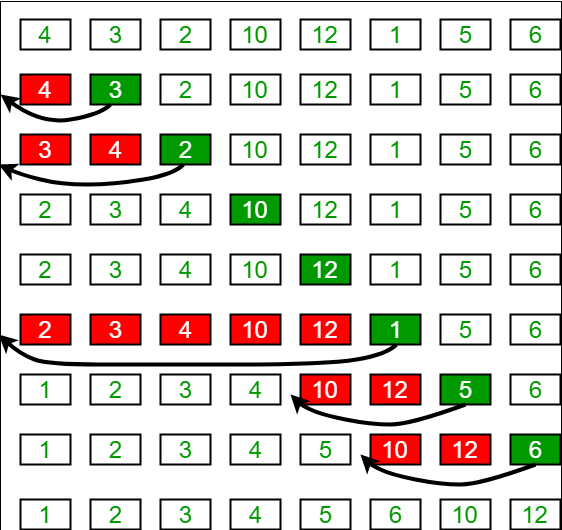
\includegraphics[width=10cm, height=6cm]{insertion-sort.png}
 \caption{Insertion Sort Execution Example}\footnotemark
    \label{fig:insertion-sort}
\end{figure}
\footnotetext{\url{https://media.geeksforgeeks.org/wp-content/uploads/insertionsort.png}}
\newline
\\
\newpage
\textbf{{\Large{Implementation}}}

\begin{lstlisting}{c++}
        #include <bits/stdc++.h>
        
        using namespace std;
        
        int n;
        void insertionSort(vector<int> &arr){
        	int key, j;
        	for (int i = 1; i < n; i++) {
        		key = arr[i];
        		j = i - 1;
        		/* Move elements of arr[0..i-1], that are
        		greater than key, to one position ahead
        		of their current position */
        		while (j >= 0 && arr[j] > key)
        		{
        			arr[j + 1] = arr[j];
        			j = j - 1;
        		}
        		arr[j + 1] = key;
        	}
        }
        int main(){
            cin >> n;
        	vector<int> arr(n);
            for(int i = 0; i < n; ++i)cin >> arr[i];
        	insertionSort(arr);
        	cout << "Array after sorting: ";
        	for(int i = 0; i < n; ++i)cout << arr[i] << " ";
        
        	return 0;
        }

\end{lstlisting}
\newpage
\section{Selection Sort $o(n^2)$}



The selection sort algorithm sorts an array by repeatedly finding the $minimum$ element (considering ascending order) from unsorted part and putting it at the beginning. The $algorithm$ maintains two $subarrays$ in a given array.\newline

1) The subarray which is already sorted.\newline
2) Remaining subarray which is unsorted.\newline

In every iteration of selection sort, the minimum element (considering ascending order) from the unsorted subarray is picked and moved to the sorted subarray.\newline
    
\textbf{{\Large{Example\footnotetext{\url{https://www.geeksforgeeks.org/selection-sort/}}}}}
\begin{lstlisting}{c++}
        arr[] = 64 25 12 22 11
        
        // Find the minimum element in arr[0...4]
        // and place it at beginning
        11 25 12 22 64
        
        // Find the minimum element in arr[1...4]
        // and place it at beginning of arr[1...4]
        11 12 25 22 64
        
        // Find the minimum element in arr[2...4]
        // and place it at beginning of arr[2...4]
        11 12 22 25 64
        
        // Find the minimum element in arr[3...4]
        // and place it at beginning of arr[3...4]
        11 12 22 25 64 

\end{lstlisting}
\\
\\
\newline\newline
\textbf{{\Large{Implementation}}}
\begin{lstlisting}{c++}
        #include <bits/stdc++.h>
        
        using namespace std;
        
        int n;
        void selectionSort(vector<int> &arr){
        	int min_idx;
        	// One by one move boundary of unsorted subarray
        	for (int i = 0; i < n-1; i++) {
        		// Find the minimum element in unsorted array
        		min_idx = i;
        		for (int j = i+1; j < n; j++)
        		if (arr[j] < arr[min_idx])
        			min_idx = j;
        
        		// Swap the found minimum element with the first element
        		swap(arr[min_idx], arr[i]);
        	}
        }
        
        int main(){
            cin >> n ;
        	vector<int> arr(n);
        	for (int i=0; i < n; i++)cin >> arr[i];
        	selectionSort(arr);
        	cout << "Sorted array: \n";
        	for (int i=0; i < n; i++)cout << arr[i] << " ";
        	return 0;
        }
\end{lstlisting}

\newpage





\section{Merge Sort $o(nlogn)$}\footnotetext{\url{https://www.hackerearth.com/practice/algorithms/sorting/merge-sort/tutorial/}}
Merge sort is a divide-and-conquer algorithm based on the idea of breaking down a list into several sub-lists until each sublist consists of a single element and merging those sublists in a manner that results into a sorted list.\newline

Idea:
\begin{itemize}
\item Divide the unsorted list into $N$ sublists, each containing  $1$ element.

\item Take adjacent pairs of two singleton lists and merge them to form a list of $2$ elements. N will now convert into $N $/$ 2$ lists of size $2$.

\item Repeat the process till a single sorted list of obtained.

\end{itemize}

\hspace{7mm}While comparing two sub-lists for merging, the first element of both lists is taken into consideration. While sorting in ascending order, the element that is of a lesser value becomes a new element of the sorted list. This procedure is repeated until both the smaller sub-lists are empty and the new combined sub-list comprises all the elements of both the sub-lists.

\textbf{\Large{Now consider the following recursive function:}}
\begin{lstlisting}{c++}
        arr[] = 64 25 12 22 11
        
        // Find the minimum element in arr[0...4]
        // and place it at beginning
        11 25 12 22 64
        
        // Find the minimum element in arr[1...4]
        // and place it at beginning of arr[1...4]
        11 12 25 22 64
        
        // Find the minimum element in arr[2...4]
        // and place it at beginning of arr[2...4]
        11 12 22 25 64
        
        // Find the minimum element in arr[3...4]
        // and place it at beginning of arr[3...4]
        11 12 22 25 64 

\end{lstlisting}
\\
\\
\newline\newline
\textbf{{\Large{Implementation}}}
\begin{lstlisting}{c++}
        void merge_sort (int A[] , int start , int end ){
            if( start < end ) {
                   int mid = (start + end ) / 2 ;// defines the current array in 2 parts .
                   merge_sort (A, start , mid ) ;// sort the 1st part of array .
                   merge_sort (A,mid+1 , end ) ;// sort the 2nd part of array.
        
                 // merge the both parts by comparing elements of both the parts.
                  merge(A,start , mid , end );   
           }                    
        }
\end{lstlisting}

\newpage

\section{Quick Sort $o(n^2)$}\footnotetext{\url{https://www.w3schools.in/data-structures-tutorial/sorting-techniques/quick-sort-algorithm/}}

Quick sort is one of the most famous sorting algorithms based on divide and conquers strategy which results in an $O$($n$$log$$n$) complexity. So, the algorithm starts by picking a single item which is called pivot and moving all smaller items before it, while all greater elements in the later portion of the list. This is the main quick sort operation named as a partition, recursively repeated on lesser and greater sub-lists until their size is one or zero - in which case the list is wholly sorted. Choosing an appropriate pivot, as an example, the central element is essential for avoiding the severely reduced performance of $o(n^2)$.
\\
\\
\newline\newline
\textbf{{\Large{Implementation}}}
\begin{lstlisting}{c++}
        #include <bits/stdc++.h>
        
        using namespace std;
        int algo(int arr[], int i, int j){
            int piv = arr[i];
            while(i < j){
                if(arr[i] > arr[j])swap(arr[i],arr[j]);
                if(piv == arr[i]){
                    j--;
                }
                else if(piv == arr[j]){
                    i++;
                }
            }
            return i;
        }
        
        void quick(int arr[], int i, int j){
            if(i < j){
               int piv = algo(arr, i, j);
               quick(arr, i, piv - 1);
               quick(arr, piv + 1, j);
            }
        }
        int main()
        {
            int arr[] = {6, 5, 4, 3, 2, 1};
            quick(arr, 0, 5);
            for(int i = 0;  i < 6; ++i)cout << arr[i] << " ";
        }

\end{lstlisting}

\chapter{Graph}

\section{Overview and Motivation} 
\label{sec:s1}
   The graph is a pervasive structure which appears in many Computer Science problems. A graph (G = (V,E)) in its basic form is simply a set of vertices (V) and edges (E; storing connectivity information between vertices in V). Later in the next section, we will explore many important graph problems and algorithms. To prepare ourselves, we will discuss three basic ways (there are a few other rare structures) to represent a graph G with V vertices and E edges in this subsection20. Many real-life problems can be classified as graph problems. Some have efficient solutions. Some do not have them yet.   
   \\
   
   In this relatively chapter, we discuss graph problems that commonly appear in real life, the algorithms to solve them, and the practical implementations of these algorithms. We cover topics ranging from basic graph traversals, minimum spanning trees, single-source/all-pairs shortest paths, and discuss graphs with special properties. In computer science, a graph is an abstract data type that is meant to implement the undirected graph and directed graph concepts from mathematics; specifically, the field of graph theory. A graph data structure consists of a finite (and possibly mutable) set of vertices (also called nodes or points), together with a set of unordered pairs of these vertices for an undirected graph or a set of ordered pairs for a directed graph. These pairs are known as edges (also called links or lines), and for a directed graph are also known as arrows. The vertices may be part of the graph structure, or may be external entities represented by integer indices or references. A graph data structure may also associate to each edge some edge value, such as a symbolic label or a numeric attribute (cost, capacity, length, etc.)in figure \ref{fig:GraphRepresentation}.
\newpage

\\
\newline
\textbf{{\Large{So, we can assume the Backtracking function as following:}}}


\begin{lstlisting}{c++}
        void backtrack(state) {
        if (hit end state or invalid state) // we need terminating or
            return; // pruning condition to avoid cycling and to speed up search
        for each neighbor of this state // try all permutation
             backtrack(neighbor);
        }
\end{lstlisting}
\\
\newline
\begin{figure}[h]
    % \centering
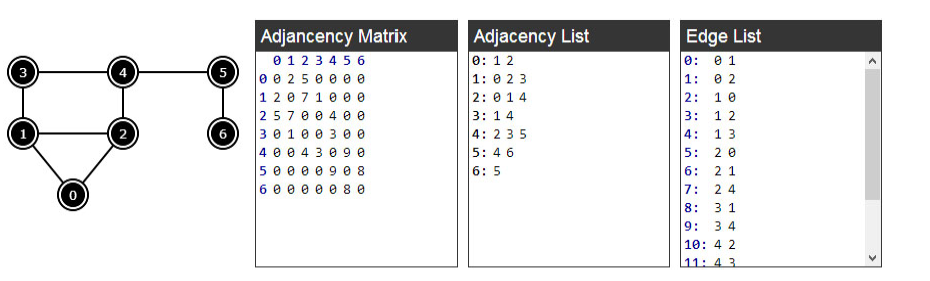
\includegraphics[width=15cm, height=5cm]{GraphRepresentation.png}
 \caption{Graph Data Structure Visualization}
    \label{fig:GraphRepresentation}
\end{figure}


\subsection{Applications}
Graph Applications appear in many problems. Like:
\begin{itemize}
\item Graph Traversing: 

Using DFS (Depth first search) and BFS (Breadth first search).
\item Finding Connected Components (Undirected Graphs) and Flood Fill -Labeling/Coloring the Connected Components-.
\item Topological Sort (Dircyed Acyclic Graph). Using DFS + stack or vector. Or Khan's Algorithm.
\item Graph Edges Property check via DFS Spanning Tree.
\item Finding Articulation Points and Bridges (Undirected Graph). \item Finding Strongly Connected Components (Directed Graph). Using Tarjan's Algorithm.
\item Finding Minimum Spanning Tree. Using Kruskal’s Algorithm and Prim’s Algorithm.
\item Finding Shortest Path Algorithms included Single-Source Shortest Paths:

SSSP on Unweighted Graph, SSSP on Weighted Graph and SSSP on Graph with Negative Weight Cycle and All-Pairs Shortest Paths -Explanation of Floyd Warshall’s DP Solution. 
\item Finding maximum flow using Edmonds Karp’s algorithm and Hopcroft Karp’s algorithm.
\end{itemize}

\newpage
\section{Graph Traversel}
This section discusses two fundamental graph algorithms: depth-first search and breadth-first search. Both algorithms are given a starting node in the graph, and they visit all nodes that can be reached from the starting node. The difference in the algorithms is the order in which they visit the nodes.
\subsection{Depth First Search (DFS) }\label{subsection:DFS}
Depth First Search is one of the main graph algorithms. Depth First Search finds the lexicographical first path in the graph from a source vertex u to each vertex. Depth First Search will also find the shortest paths in a tree (because there only exists one simple path), but on general graphs this is not the case. The algorithm works in O(m+n) time where n is the number of vertices and m is the number of edges.

\subsubsection{Example}\ref{subsection:DFS}
Let us consider how depth-first search processes the following graph:

\begin{figure}[h]
    \centering
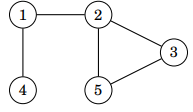
\includegraphics[width=5cm, height=3cm]{graph-example.png}
 \caption{Sample Graph}
    \label{fig:graph-example}
\end{figure}

We may begin the search at any node of the graph. So, let's start traversing at node 1. After that, searching will traversing node 2:

\begin{figure}[h]
    \centering
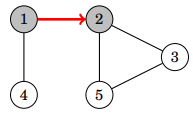
\includegraphics[width=5cm, height=3cm]{graph-example-traverse-1.png}
 \caption{step 1: Sample Graph After Traversing}
    \label{fig:graph-example-traverse-1}
\end{figure}

\newpage

After this, nodes 3 and 5 will be visited:

\begin{figure}[h]
    \centering
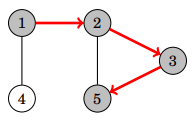
\includegraphics[width=5cm, height=3cm]{graph-example-traverse-2.png}
 \caption{step 2: Sample Graph After Traversing}
    \label{fig:graph-example-traverse-2}
\end{figure}

The neighbors of node 5 are 2 and 3, but the search has already visited both of them, so it is time to return to the previous nodes. Also the neighbors of nodes 3 and 2 have been visited, so we next move from node 1 to node 4:

\begin{figure}[h]
    \centering
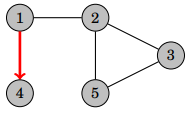
\includegraphics[width=5cm, height=3cm]{graph-example-traverse-3.png}
 \caption{step 3: Sample Graph After Traversing}
    \label{fig:graph-example-traverse-3}
\end{figure}

After this, the search terminates because it has visited all nodes.
The time complexity of depth-first search is O(n+ m) where n is the number of nodes and m is the number of edges, because the algorithm processes each node and edge once.
\newpage

\subsubsection{Implementation}

Depth-first search can be conveniently implemented using recursion. The following function dfs begins a depth-first search at a given node. The function assumes that the graph is stored as adjacency lists in an array, so the following representation is array of vectors: 
\begin{lstlisting}{c++}
        vector<int> adj[N]; //vector< vector<int> > adj; //int adj[N][N];
\end{lstlisting}

Also, we will maintain a visited array to avoid cycles:
\begin{lstlisting}{c++}
        bool visited[N]; //To not visit node more than one time
\end{lstlisting}

The following function will keep get source node, or the start node to start traversing via the graph nodes, such that the visited array keeps track of the visited nodes. Initially, each array value is false, and
when the search arrives at node s, the value of visited[s] becomes true. The function can be implemented as follows:
\begin{lstlisting}{c++}
        typedef vector<int> vi; //vi is abbreviation for vector<int>
        bool visited; //global variable, initially all values are set to false
        void dfs(int s) { // DFS for normal usage: as graph traversal algorithm
                visited[s] = true;// important: we mark this vertex as visited
                for (int j = 0; j < (int)AdjList[s].size(); j++) { // default DS: AdjList
                int child = AdjList[s][j]; //child is a (neighbor) for his parent -parent is the node current node in upper bound level-
                if (visited[child] == false) //important check to avoid cycle
                    dfs(chlid); //recursively visits unvisited neighbors of vertex chlid, and child will be a parent for its neighboors
        } }
\end{lstlisting}
It is the same as the previous functon, but changing just two lines to of this code to be fammiliar more and more with the code:
\begin{lstlisting}{c++}
        typedef vector<int> vi; //vi is abbreviation for vector<int>
        vector<bool> visited; //global variable, initially all values are set to false
        void dfs(int s) { // DFS for normal usage: as graph traversal algorithm
                if (visited[s]) return;//important check to avoid cycle
                visited[s] = true;//important: we mark this vertex as visited
                for (int j = 0; j < (int)AdjList[s].size(); j++) { // default DS: AdjList
                int child = AdjList[s][j]; //child is a (neighbor) for his parent -parent is the node current node in upper bound level-
                    dfs(chlid); //recursively visits unvisited neighbors of vertex chlid, and child will be a parent for its neighboors
        } }
\end{lstlisting}




But for an awesome small words of codes. We can get some help from benefits of c++14, to change the syntax to be a bit samller than before:
\begin{lstlisting}{c++}
        void dfs(int s) {
                if (visited[s]) return; //important check to avoid cycle and if the current node was visited BACKTRACK 
                visited[s] = true;//important: we mark this vertex as visited
                // process node s
                for (auto child: adj[s]) {
                       dfs(child);
                }
        }
\end{lstlisting}
\newpage 
But also, it is the same as the previous functon, but changing just two lines to of this code to be fammiliar more and more with the code:
\begin{lstlisting}{c++}
        void dfs(int s) {
                 //if the current node was visited BACKTRACK 
                visited[s] = true//important: we mark this vertex as visited
                // process node s
                for (auto child: adj[s]) {
                    if(!visited[child])//important check to avoid cycle and if the current node was visited BACKTRACK 
                       dfs(child);
                }
        }
\end{lstlisting}

\newpage 

\subsection{Breadth First Search (BFS)}\label{subsec:BFS}
Breadth-first search (BFS) is one of the basic and essential searching algorithms on graphs. BFS visits the nodes in increasing order of their distance from the starting node. Thus, we can calculate the distance from the starting node to all other nodes using breadth-first search. Breadth-first search goes through the nodes one level after another. First the search explores the nodes whose distance from the starting node is 1, then the nodes whose distance is 2, and so on. This process continues until all nodes have been visited.\\
More precisely, the algorithm can be stated as follows: Create a queue q which will contain the vertices to be processed and a Boolean array used[] which indicates for each vertex, if it has been lit (or visited) or not.

Initially, push the source s to the queue and set used[s]=true, and for all other vertices v set used[v]=false. Then, loop until the queue is empty and in each iteration, pop a vertex from the front of the queue. Iterate through all the edges going out of this vertex and if some of these edges go to vertices that are not already lit, set them on fire and place them in the queue.

As a result, when the queue is empty, the "ring of fire" contains all vertices reachable from the source s, with each vertex reached in the shortest possible way. You can also calculate the lengths of the shortest paths (which just requires maintaining an array of path lengths d[]) as well as save information to restore all of these shortest paths (for this, it is necessary to maintain an array of "parents" p[], which stores for each vertex the vertex from which we reached it).   
\subsubsection{Example}
\begin{figure}[h]
    \centering
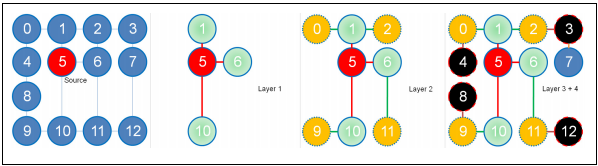
\includegraphics[width=16cm, height=4cm]{BFS-animation.png}
 \caption{Example Animation of BFS.}
    \label{fig:BFS-animation}
\end{figure}

If we run BFS from vertex 5 (i.e. the source vertex s = 5) on the connected undirected
graph shown in Figure 4.3, we will visit the vertices in the following order:

Layer 0: visit 5. Layer 1: visit 1, visit 6, visit 10. Layer 2: visit 0, visit 2, visit 11, visit 9. Layer 3: visit 4, visit 3, visit 12, visit 8. Layer 4: visit 7

\subsubsection{Implementation}
We write code for the described algorithm in C++ to traverse the previous given graph:
\begin{lstlisting}{c++}
        int nodes; //number of nodes
        int source; //source vertex
        
        queue<int> q;
        vector<bool> visited(nodes); //bool used[nodes]; 
        vector< vector<int> > adj;  //adjacency list representation
        //vector<int> adj[n]; as the same as vector< vector<int> > adj;
        q.push(source);
        visited[source] = true; //Source node marked as visited
        while (!q.empty()) {
            int v = q.front();
            q.pop();
            for (int u : adj[v]) {
                if (!used[u]) {
                    visited[u] = true;
                    q.push(u);
                }
            }
            /*
            for (int j = 0; j < adj[v].size(); j++) {
                int child =  adj[v][j];
                if (!visited[child]) {
                    visited[child] = true;
                    q.push(child);
                }
            }
            */
        }
\end{lstlisting}

\newpage

\subsection{Task Assignment Problem (Topological Sort -DAG-)}
Topological sorting of vertices of a Directed Acyclic Graph is an ordering of the vertices $v_1, v_2, ... v_n$ in such a way, that if vertex $u$ comes before vertex $v$ $(u $ → $ v)$ exists in the DAG. 
exists in the DAG. Every DAG has at least one and possibly more topological sort(s). One application of topological sorting is to find a possible sequence of curriculum that a University student has to take to fulfill graduation requirement. Each curricula has certain pre-requisites to be met. These pre-requisites are never cyclic, so they can be modeled as a DAG. Topological sorting this module pre-requisites DAG gives the student a linear list of curriculum be taken one after another without violating the pre-requisites constraints. In order to have a topological sorting the graph must not contain any cycles. In order to prove it, let's assume there is a cycle made of the vertices $v_1, v_2, v_3 ... v_n$. That means there is a directed edge between $v_i$ and $v_{i+1}$ $(1 \le i \lt< n)$ and between $v_n$ and $v_1$. So now, if we do topological sorting then $v_n$ must come before $v_1$ because of the directed edge from $v_n$ to $v_1$. Clearly, $v_{i+1}$ will come after $v_i$, because of the directed from $v_i$ to $v_{i+1}$, that means $v_1$ must come before $v_n$. Well, clearly we've reached a contradiction, here. So topological sorting can be achieved for only directed and acyclic graphs. Like the following figure \ref{fig:topo-sort}
\begin{figure}[h]
    \centering
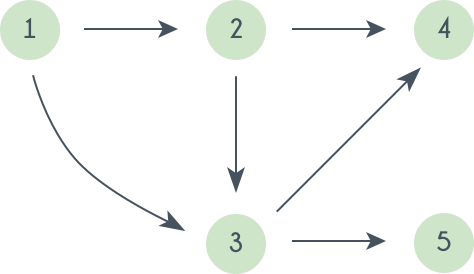
\includegraphics[width=10cm, height=6cm]{topo-sort.png}
 \caption{An Example of Topological Sort (DAG)}\footnotemark
    \label{fig:topo-sort}
\end{figure}
\footnotetext{\url{https://www.hackerearth.com/practice/algorithms/graphs/topological-sort/tutorial/}}

A topological sorting of this graph is: $1$ $2$ $3$ $4$ $5$

There are multiple topological sorting possible for a graph. For the graph given above one another topological sorting is: $1$ $2$ $3$ $5$ $4$

To implement the idea of Topological Sort. There are several algorithms for topological sort. The simplest way is to slightly modify the DFS implementation we presented earlier in subsection \ref{subsection:DFS}.

\newpage

\begin{lstlisting}{c++}
        int nodes;
        stack<int> topsort;
        vector<bool> visited;
        vector< vector<int> > adj;
        void dfs(int node){
        
        	visited[node] = true;
        
        	for(int i = 0; i < adj[node].size(); ++i){
        		int child = adj[node][i];
        		if (!visited[child])	// To avoid cyclic behavior
        			dfs(child);
        	}
        
        	topsort.push(node);// DAG //Possibly, we can use vector to push values in, and reverse it in main function.
        }
\end{lstlisting}

\newpage

\section{Single-Source Shortest Paths}\label{sec:Single-Source Shortest Paths}
\subsection{ Overview and Motivation}
Motivating problem: Given a \textbf{weighted graph} $G$ and a starting source vertex $s$, what are the \textbf{shortest paths} from s to every other vertices of $G$?

\hspace{7mm} This problem is called the \textbf{Single-Source Shortest Paths (SSSP)} problem on a \textbf{weighted graph}. It is a classical problem in graph theory and has many real life applications. For example, we can model the city that we live in as a graph. The vertices are the road junctions. The edges are the roads. The time taken to traverse a road is the weight of the edge. You are currently in one road junction. What is the shortest possible time to reach another certain road junction?

\hspace{7mm}There are efficient algorithms to solve this \textbf{SSSP} problem. If the graph is \textbf{unweighted} (or all edges have equal or constant weight), we can use the efficient \textbf{$O(V + E)$} \textbf{BFS} algorithm shown earlier in subsection \ref{subsec:BFS}. For a general weighted graph, BFS does not work correctly and we should use algorithms like the {$O((V + E) log V )$} \textbf{Dijkstra’s} algorithm or the \textbf{$O(V E)$} \textbf{Bellman Ford’s} algorithm. These various algorithms are discussed below.

\subsection{SSSP on Unweighted Graph}\label{subsec:SSSP on Unweighted Graph}
Let’s revisit subsection \ref{subsec:BFS}. The fact that BFS visits vertices of a graph layer by layer or level by level from a source vertex (see Figure \ref{fig:BFS-animation}).Inan unweighted graph, the distance between two neighboring vertices connected with an edge is simply one unit (constant value).Therefore, the layer count of a vertex that we have seen in subsection \ref{subsec:BFS} is precisely the shortest path length from the source to that vertex. For example in Figure \ref{fig:BFS-animation} the shortest path from vertex 5 to vertex 7, is 4, as 7 is in the fourth layer in BFS sequence of visitation starting from vertex 5.\\
\indent Some programming problems require us to reconstruct (restore - print) the actual shortest path, not just the shortest path length. For example, in Figure \ref{fig:BFS-animation}the shortest path from $5$ to $7$ is $5$ → $1$ → $2$ → $3$ → $7$. This can be easily done using vector of integers $vector<int> parent$. Each vertex $v$ remembers its parent $u$ $(p[v] = u)$.  For this example, vertex $7$ remembers $3$ as its parent, vertex $3$ remembers $2$, vertex $2$ remembers $1$, vertex $1$ remembers $5$ (the source). To reconstruct the actual shortest path, we can do a simple recursion from the last vertex $7$ until we hit the source vertex $5$. The modified BFS code (check the comments) is relatively simple:

\begin{lstlisting}{c++}
        #define INF (int)INT_MAX
        void printPath(int u) { // extract information from              vector<int> p
            if (u == source) { cout << source; return; } // base case, at the source s
            printPath(p[u]); // recursive: to make the output format: s -> ... -> t
            cout << u; 
        }
         int main()
            vector<int> dist(V, INF); dist[source] = 0; // distance from source s to s is 0
            queue<int> q; q.push(source);
            vector<int> p; // addition: the predecessor/parent vector
            while (!q.empty()) {
                int u = q.front(); q.pop();
                for (int j = 0; j < (int)AdjList[u].size(); j++) {
                int child = AdjList[u][j];
                if (dist[child] == INF) {
                        dist[child] = dist[u] + 1;
                        p[child] = u; // addition: the parent of vertex child is u
                        q.push(child);
                    }
                }
            }
            printPath(t), cout << endl; // addition: call printPath from vertex t

\end{lstlisting}

\newpage

\subsection{SSSP on Weighted Graph}\label{subsec:SSSP on Weighted Graph}
If the given graph is weighted, BFS does not work. This is because there can be ‘longer’ path(s) (in terms of number of vertices and edges involved in the path) but has smaller total weight than the ‘shorter’ path found by BFS. For example, in Figure \ref{fig:dijkstra-animation}.

\begin{figure}[h]
    \centering
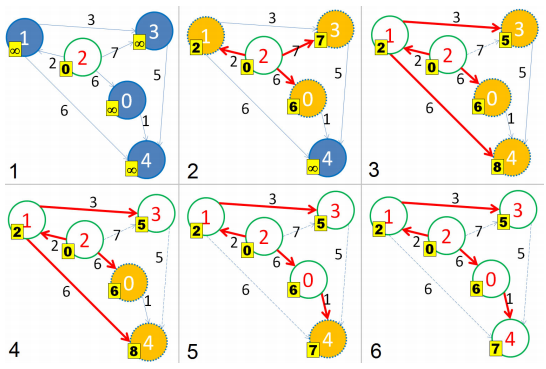
\includegraphics[width=10cm, height=6cm]{dijkstra-animation.png}
 \caption{Dijkstra Animation on a Weighted Graph (from \href{https://vj.z180.cn/52627383937f06635b950dd1efa17b6a?v=1575637256}{\color{red}{UVa 341}})}
    \label{fig:dijkstra-animation}
\end{figure}
\\
\hspace{7mm}The shortest path from source vertex 2 to vertex 3 is not via direct edge 2 → 3 with weight 7 that is normally found by BFS, but a ‘detour’ path: 2 → 1 → 3 with smaller total weight 2 + 3 = 5.

\hspace{7mm}To solve the SSSP problem on weighted graph, we use a greedy Edsger Wybe $Dijkstra’s$ algorithm. There are several ways to implement this classic algorithm. Here we adopt one of the easiest implementation variant that uses built-in C++ STL \lstinline|priority_queue| (or Java \lstinline|PriorityQueue|). This is to keep the length of code minimal—a necessary feature in complexty and programming.

\hspace{7mm}This $Dijkstra’s$ variant maintains a priority queue called $pq$ that stores pairs of vertex
information. The first and the second item of the pair is the distance of the vertex from the
source and the vertex number, respectively. This $pq$ is sorted based on increasing distance
from the source, and if tie, by vertex number.

\hspace{7mm}This \lstinline|pq| only contains one item initially: The base case ($0$, $s$) which is true for the source
vertex. Then, this $Dijkstra’s$ implementation variant repeats the following process until \lstinline|pq|
is empty: It greedily takes out vertex information pair ($d$, $u$) from the front of \lstinline|pq|. If the
distance to $u$ from source recorded in d greater than \lstinline|dist[u]|, it ignores $u$; otherwise, it
process $u$. The reason for this special check is shown below.

\hspace{7mm}When this algorithm process $u$, it tries to relax \footnotemark 
\footnotetext{The operation: relax(u, v, weight-u-v) sets dist[v] = min(dist[v], dist[u] + weight-u-v).}
all neighbors $v$ of $u$. Every time it
relaxes an edge $u$ → $v$, it will enqueue a pair (newer/shorter distance to $v$ from source, $v$)
into \lstinline|pq| and leave the inferior pair (older/longer distance to $v$ from source, $v$) inside \lstinline|pq|. This
is called ‘Lazy Deletion’ and it causes more than one copy of the same vertex in \lstinline|pq| with
different distances from source. That is why we have the check earlier to process only the
first dequeued vertex information pair which has the correct/shorter distance (other copies
will have the outdated/longer distance). The code is shown below and it looks very similar
to BFS code shown in subection \ref{subsec:BFS}\newline\newline

\textbf{{\Large{Dijkstra Animation}}}\newline
\begin{figure}[h]
    \centering
\includegraphics[width=10cm, height=6cm]{DijkstraAnimation.gif}
 \caption{Dijkstra Animation on a Weighted Graph (\href{https://upload.wikimedia.org/wikipedia/commons/5/57/Dijkstra_Animation.gif}{\color{blue}{\textbf{Link}}})}
    \label{fig:DijkstraAnimation}
\end{figure}
\\
\newline

\textbf{{\Large{Implementation}}}\newline
\begin{lstlisting}{c++}
        #include<bits/stdc++.h>
        using namespace std;
        
        typedef pair<int, int> ii;
        typedef vector<int> vi;
        typedef vector<ii> vii;
        #define INF INT_MAX
        
        int main() {
          int V, E, s, u, v, w;
          vector<vii> AdjList;
        
          /*
          // Graph in Figure 2.8
          5 7 2
          2 1 2
          2 3 7
          2 0 6
          1 3 3
          1 4 6
          3 4 5
          0 4 1
          */
        
          cin >> V >> E >> s;
        
          AdjList.assign(V, vii()); // assign blank vectors of pair<int, int>s to AdjList
          for (int i = 0; i < E; i++) {
            cin >> u >> v >> w;
            AdjList[u].push_back(ii(v, w));// directed graph
          }
        
          // Dijkstra routine
          vi dist(V, INF); dist[s] = 0; // INF = INT_MAX to avoid overflow
          priority_queue< ii, vector<ii>, greater<ii> > pq; pq.push(ii(0, s)); // (^_|_^) to sort the pairs by increasing distance from s
          while (!pq.empty()) { // main loop
            ii front = pq.top(); pq.pop(); // greedy: pick shortest unvisited vertex
            int d = front.first, u = front.second;
            if (d > dist[u]) continue; // this check is important, see the explanation
            for (int j = 0; j < (int)AdjList[u].size(); j++) {
              ii v = AdjList[u][j]; // all outgoing edges from u
              if (dist[u] + v.second < dist[v.first]) {
                dist[v.first] = dist[u] + v.second;// relax operation
                pq.push(ii(dist[v.first], v.first));
          } } }// note: this variant can cause duplicate items in the priority queue
        
          for (int i = 0; i < V; i++) // index + 1 for final answer
            cout << SSSP( << s << , << i << ) << = << dist[i] << endl;
        
          return 0;
        }
\end{lstlisting}


\chapter{Problem Solving Paradigms}
\label{chap:ProblemSolvingParadigms}

\section{Overview and Motivation}

\large{\upshape{As commonly known or almost problem solving paradigms that is known, four problem solving paradigms. So in this chapter, we will discuss  commonly used namely like: Complete Search (a.k.a Brute Force), Divide and Conquer, the Greedy approach, and Dynamic Programming.}}
\\
\newline
\textbf{{\Large{So, we can assume the Backtrackig function as following:}}}


\begin{lstlisting}{c++}
        void backtrack(state) {
        if (hit end state or invalid state) // we need terminating or
            return; // pruning condition to avoid cycling and to speed up search
        for each neighbor of this state // try all permutation
             backtrack(neighbor);
        }
\end{lstlisting}

\newpage


\section{8-Queen Problem (Recursive Complete Search -Backtracking-)}
\label{8-Queen}

\href{https://vj.z180.cn/a1d3d6853584bb15ac7da3eeee0977ca?v=1575822738}{\color{red}{\textbf {UVa 750}}}\textbf{ - 8 Queens Chess Problem}

\begin{figure}[h]
    \centering
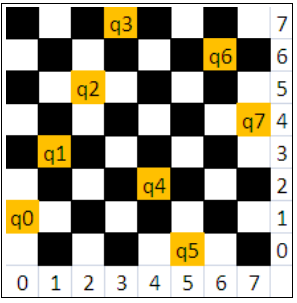
\includegraphics[width=6cm, height=6cm]{8-queen-problem.png}
 \caption{\textbf{8-Queens problem competitive programming 3, p.74}}
    \label{fig:8-queen-problem}
\end{figure}

Abridged problem statement: In chess (with an $8$ × $8$ board), it is possible to place eight queens on the board such that no two queens attack each other. Determine all such possible arrangements given the position of one of the queens (i.e. coordinate ($a$, $b$) must contain a queen). Output the possibilities in $lexicographical$ (sorted) order.
\\

\hspace{7mm}The most naive solution is to enumerate all combinations of 8 different cells out of the
8 × 8 = 64 possible cells in a chess board and see if the 8 queens can be placed at these positions without conflicts. However, there are $_6_4C_8$ $\approx$ $4B$ such possibilities—this idea is not even worth trying.
\\
 
\hspace{7mm}A better but still naive solution is to realize that each queen can only occupy one column, so we can put exactly one queen in each column. There are only $8^8$ $\approx$ $17M$ possibilities now,
down from $4B$. This is still a ‘borderline’-passing solution for this problem. If we write a Complete Search like this, we are likely to receive the Time Limit Exceeded (TLE) verdict especially if there are multiple test cases. We can still apply the few more easy optimizations described below to further reduce the search space.

\hspace{7mm}We know that no two queens can share the same column or the
same row. Using this, we can further simplify the original problem
to the problem of finding valid permutations of 8! row positions.
The value of \lstinline|row[i]| describes the row position of the queen in
column i. Example: \lstinline|row = {1, 3, 5, 7, 2, 0, 6, 4}| as in Figure\ref{fig:8-queen-problem} is one of the solutions for this problem;  \lstinline|row[0] = 1| implies that the queen in column 0 is placed in row 1, and so on (the index starts from 0 in this example). Modeled this way, the search space goes down from $8^8$ $\approx$ $17M$ to $8!$ $\approx$ $40K$  This solution is already fast enough, but we can still do more.
\\

\hspace{7mm}We also know that no two queens can share any of the two diagonal lines. Let queen A be at \lstinline|(i, j)| and queen B be at \lstinline|(k, l)|. They attack each other if \lstinline|abs(i-k) == abs(j-l)|. This formula means that the vertical and horizontal distances between these two queens are equal, i.e. queen A and B lie on one of each other’s two diagonal lines.
\\

\hspace{7mm}A recursive backtracking solution places the queens one by one in columns 0 to 7, observing all the constraints above. Finally, if a candidate solution is found, check if at least one of the queens satisfies the input constraints, i.e. \lstinline|row[b] == a|. This sub (i.e. lower than) $O(n!)$ solution will obtain an AC verdict.
\\

\begin{lstlisting}{c++}
        /* 8 Queens Chess Problem */
        #include<bits/stdc++.h>
        
        using namespace std;
        
        int row[8], TC, a, b, lineCounter; //ok to use global variables
        
        bool place(int r, int c) {
          for (int prev = 0; prev < c; prev++) //check previously placed queens
            if (row[prev] == r || (abs(row[prev] - r) == abs(prev - c)))
              return false;//share same row or same diagonal -> infeasible
          return true; }
        
        void backtrack(int c) {
          if (c == 8 && row[b] == a) {// candidate sol, (a, b) has 1 queen
            cout << ++lineCounter << "      " << row[0] + 1;
            for (int j = 1; j < 8; j++)cout << row[j] + 1;
            cout << endl; }
          for (int r = 0; r < 8; r++) // try all possible row
            if (place(r, c)) {//if can place a queen at this col and row
              row[c] = r; backtrack(c + 1); // put this queen here and recurse
        }   }
        
        int main() {
          cni >> TC;
          while (TC--) {
            cin >> a >> b; a--; b--;//switch to 0-based indexing
            memset(row, 0, sizeof row); lineCounter = 0;
            cout << SOLN <<         << COLUMN << endl;
            cout << # <<      << 1 2 3 4 5 6 7 8 << endl << endl;
            backtrack(0); //generate all possible 8! candidate solutions
            if (TC)cout << endl;
        } }   

\end{lstlisting}

\clearpage


\section{N-queen Problem (More Challenging Backtracking)}
\label{n-Queen}

\href{https://vj.z180.cn/7e4e8d92abc27cb470b49794bd31bb31?v=1575831964}{\color{red}{\textbf {UVa 11195}}}\textbf{ - N Queens Chess Problem}

\begin{figure}[h]
    \centering
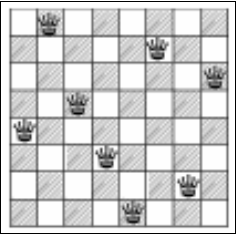
\includegraphics[width=6cm, height=6cm]{n-queen-problem.png}
 \caption{\textbf{N-Queens problem UVa 11195}}
    \label{fig:n-queen-problem}
\end{figure}

Abridged problem statement: Given an $n$ × $n$ chessboard ($3$ $<$ $n$ $<$ $15$) where some of the cells are bad (queens cannot be placed on those bad cells), how many ways can you place $n$ queens in the chessboard so that no two queens attack each other? Note: Bad cells cannot be used to block queens’ attack.

\hspace{7mm}The recursive backtracking code that we have presented above is not fast enough for $n = 14$ and no bad cells, the worst possible test case for this problem. The $sub-O(n!)$ solution presented earlier is still OK for $n = 8$ but not for $n$ = 14. We have to do better. The major issue with the previous $n$-queens code is that it is quite slow when checking whether the position of a new queen is valid since we compare the new queen’s position with the previous \lstinline|c-1| queens’ positions (see function \lstinline|bool place(int r, int c)|).

\hspace{7mm}Initially all n rows (rw), 2 × n − 1 left diagonals (ld), and 2 × n − 1 right diagonals (rd) are unused (these three bitsets are all set to false). When a queen is placed at cell (r, c), we flag rw[r] = true to disallow this row from being used again. Furthermore, all (a, b) where abs(r - a) = abs(c - b) also cannot be used anymore. There are two possibilities after removing the abs function: r-c=a-b and r+c=a+b. Note that r+c and r-c represent indices for the two diagonal axes. As r-c can be negative, we add an offset of n-1 to both sides of the equation so that r-c+n-1=a-b+n-1. If a queen is placed on cell (r, c), we flag ld[r - c + n - 1] = true and rd[r + c] = true to disallow these two diagonals from being used again. With these additional data structures and the additional problem-specific constraint in UVa 11195 (board[r][c] cannot be a bad cell), we can extend our code to become:

\begin{lstlisting}{c++}
        void backtrack(int c) {
        if (c == n) { ans++; return; } // a solution
        for (int r = 0; r < n; r++) // try all possible row
            if (board[r][c] != ’*’ && !rw[r] && !ld[r - c + n - 1] && !rd[r + c]) {
            rw[r] = ld[r - c + n - 1] = rd[r + c] = true; // flag off
            backtrack(c + 1);
            rw[r] = ld[r - c + n - 1] = rd[r + c] = false; // restore
        } }
\end{lstlisting}

\newpage
%\section{8-queen \& N-queen Problem Using Bitmask}

\section{Dynamic Programming}\label{sec:dp}
\subsection{Overview and Motivation}
Dynamic Programming (from now on abbreviated as DP) is perhaps the most challenging problem-solving technique among the four paradigms. The key skills that you have to develop in order to master DP are the abilities to determine the problem states and to determine the relationships or transitions between current problems and their sub-problems. We have used these skills earlier in recursive backtracking (see Section \ref{n-Queen} \& \ref{8-Queen}). In fact, DP problems with small input size constraints may already be solvable with recursive backtracking. DP is primarily used to solve optimization problems and counting problems. If you encounter a problem that says “minimize this” or “maximize that” or “count the ways to do that”, then there is a (high) chance that it is a DP problem. Most DP problems ask for the optimal/total value and not the optimal solution itself, which often makes the problem easier to solve by removing the need to backtrack and produce the solution. However, some harder DP problems also require the optimal solution to be returned in some fashion. We will continually refine our understanding of Dynamic Programming in this section.

\subsection{Knapsack Problem (0/1 Knapsack)}
Also called subset sum. So the problem is, he is a thief, who has a bag. This bag has a specific weight. He will enter a house and will steal things from this house. Everything has a specific weight and value he knows it. For example, he can take a gold ring. Although it is very light, it has a high benefit or a high value. And he can steal T.V. Although it has a low value, it has a high weight. The problem asks you, which items he can take, such that, these the weight of items fit in this bag + benefit of these items have a high cost as possible? 

\hspace{7mm}This problem is called.  This problem is also called 0/1 knapsack. It means that this item will be picked or it will be left -pick or leave-.
\newpage
\begin{figure}[h]
    \centering
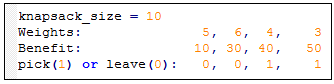
\includegraphics[width=14cm, height=3cm]{knapsack-example-1.png}
 \caption{\textbf{Knapsack Example 1}}
    \label{fig:knapsack-example-1}
\end{figure}
\\
\hspace{7mm}A cursory look at the example data tells us that the max value that we could accommodate with the limit of max weight of 10 is 50 + 40 = 90 with a weight of 7. 

\begin{figure}[h]
    \centering
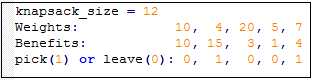
\includegraphics[width=14cm, height=3cm]{knapsack-example-2.png}
 \caption{\textbf{Knapsack Example 2}}
    \label{fig:knapsack-example-2}
\end{figure}
\\
\hspace{7mm}Also, a cursory look at the example data tells us that the max value that we could accommodate with the limit of max weight of 10 is 15 + 4 = 19 with a weight of 11.
\subsubsection{Recursion Implementation}
\begin{lstlisting}{c++}
        #include <bits/stdc++.h>
        #define INF INT_MIN
        
        using namespace std;
        
        struct item{
        	int weight;
        	int benefit;
        };
        
        int noOfItems;
        vector<item> items;
        int knapsack01(int index, int reminder) {
        	if (reminder < 0)return -INF;
        	if (reminder == 0 || index == noOfItems)return 0;
        	int Choice1 = knapsack01(index + 1, reminder);///I don't take the item, so i will go the next one i + 1. And the weight will still unchanged in the bag,
        	int Choice2 = knapsack01(index + 1, reminder - items[index].weight) + items[index].benefit;///After we take the item, i will go to the one after me, and i will remove the weight that i take it so far.
        	return max(Choice1, Choice2);
        }
        
        int main() {
        	ios_base::sync_with_stdio(0), cin.tie(0), cout.tie(0);
        	int tests; cin >> tests;
        	while (tests--) {
        		int weights;
        		cin >> noOfItems >> weights;
        		items = vector<item>(noOfItems);
        		for (int i = 0; i < noOfItems; i++)cin >> items[i].weight;
        		for (int i = 0; i < noOfItems; i++)cin >> items[i].benefit;
        		cout << knapsack01(0, weights) << endl;
        	}
        }
\end{lstlisting}

\subsubsection{DP (Top Down Approach) Implementation}
\begin{lstlisting}{c++}
        #include <bits/stdc++.h>
        #define INF INT_MIN
        
        using namespace std;
        
        struct item{
        	int weight;
        	int benefit;
        };
        
        const int MAX = 1001;
        int mem[MAX][MAX];
        int noOfItems;
        vector<item> items;
        
        int knapsack01(int index, int reminder) {
        	if (reminder < 0)return -INF;
            if (reminder == 0 || index == noOfItems)return 0;
        	int& bestChoice = mem[index][reminder];
        	if (~bestChoice)return bestChoice; ///as the same as, if (bestChoice != -1)
        	bestChoice = knapsack01(index + 1, reminder);///I don't take the item, so i will go the next one i + 1. And the weight will still unchanged in the bag,
        	bestChoice = max(bestChoice, knapsack01(index + 1, reminder - items[index].weight) + items[index].benefit);///After we take the item, i will go to the one after me, and i will remove the weight that i take it so far.
        	return bestChoice;
        }
        
        int main() {
        	ios_base::sync_with_stdio(0), cin.tie(0), cout.tie(0);///To fast input and output
        	int tests; cin >> tests;
        	while (tests--){
                int weights;
                cin >> noOfItems >> weights;
                items = vector<item>(noOfItems);
                for (int i = 0; i < noOfItems; i++)cin >> items[i].weight;
                for (int i = 0; i < noOfItems; i++)cin >> items[i].benefit;
                cout << knapsack01(0, weights) << endl;
            }
        }
\end{lstlisting}

\newpage

\subsection{Traveling Sales Man Problem (TSP)}
Problem: Given $n$ cities and their pairwise distances in the form of a matrix dist of size $n$ × $n$, compute the cost of making a tour18 that starts from any city $s$, goes through all the other $n$ − 1 cities exactly once, and finally returns to the starting city $s$.

\begin{figure}[h]
    \centering
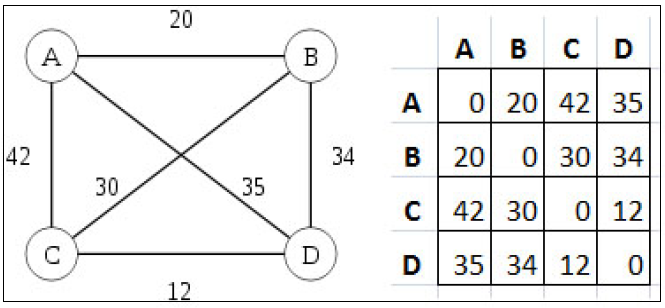
\includegraphics[width=14cm, height=7cm]{TSP.png}
 \caption{Complete Graph To Visualize TSP, \textbf{CP 3 book}}
    \label{fig:TSP}
\end{figure}

\hspace{7mm}Example: The graph shown in Figure \ref{TSP} has $n$ = 4 cities. Therefore, we have 4! = 24 possible tours (permutations of 4 cities). One of the minimum tours is \textbf{A-B-C-D-A} with a cost of \textbf{20+30+12+35 = 97} (notice that there can be more than one optimal solution).

\hspace{7mm}A ‘brute force’ TSP solution (either iterative or recursive) that tries all $O((n - 1)!)$ possible tours (fixing the first city to vertex A in order to take advantage of symmetry as the graph is undirected) is only effective when $n$ is at most $12$ as 11 $!$$\approx$ 40$M$. When $n$$>$12, such brute force solutions will
get a TLE in \textbf{Online Judges}. However, if there are multipl test cases, the limit for such ‘brute force’ TSP solution is probably just $n$ = 11.

\hspace{7mm}We can utilize DP for TSP since the computation of sub-tours is clearly overlapping, e.g. the tour \textbf{A - B - C - (n - 3)} other cities that finally return to A clearly overlaps the tour \textbf{A - C - B - the same (n - 3)} other cities that also return to A. If we can avoid re-computing the lengths of such \textbf{sub-tours}, we can save a lot of computation time. However, a distinct state in TSP depends on two parameters: The last \textbf{city/vertex} visited pos and something that we may have not seen before—a subset of visited cities.

\hspace{7mm}There are many ways to represent a set. However, since we are going to pass this set
information around as a parameter of a recursive function (if using top-down DP), the representation we use must be lightweight and efficient! In Section \ref{sec:dp}. If we have $n$ cities, we use a binary integer of length n. If bit i is ‘1’ (on), we say that item (city) $i$ is inside the set (it has been visited) and item $i$ is not inside the set (and has not been visited) if the bit is instead $‘0’$ (off). For example: mask= 1810 = 100102 implies that items (cities) {1, 4} are in19 the set (and have been visited). Recall that to check if bit $i$ is on or off, we can use \lstinline|{mask & (1 << i)}|. To set bit $i$, we can use \lstinline{mask |= (1 << i)} .

\begin{lstlisting}{c++}
        const int INF = 1e9;
        int BottomUp(vector<vector<int> > dist) { //Distance between city(i,j);
            int n = dist.size();
            int lim = 1 << n; //It means, 2 to the power n
            int dp[lim][n];
            memset(dp, INF, sizeof(dp));
            for (int i = 0; i < n; i++) {
                dp[1 << i][i] = 0;    // base case of visiting just 1 city
            }
            for (int mask = 0; mask < lim; mask++) {
                for (int last = 0; last < n; last++) {
                    if (mask & (1 << last) == 0) { // Didn't visit last.
                        continue;
                    }
                    for (int curr = 0; curr < n; curr++) {
                        if (mask & (1 << curr) == 0) { // Didn't visit current
                            continue;
                        }
                        int otherMask = mask ^ (1 << curr);
                        dp[mask][curr] = min(dp[mask][curr], dp[otherMask][last] + dist[last][curr]);
                    }
                }
            }
            int ans = INF;
            for (int i = 0; i < n; i++) {
                ans = min(ans, dp[lim - 1][i]);
            }
            return ans;
        }
        
        int memo[][];
        int TopDown(int pos,int mask){
          if (mask == (1 << V) - 1)
        			return cost[pos][0];
          if (memo[pos][mask]!=-1) {
            return memo[pos][mask];
          }
        		int min = INF;
        		for (int nxt = 0 ; nxt < V ; ++nxt)
        			if (nxt != pos && (mask & (1 << nxt)) == 0)
        				min = Math.min(min, cost[pos][nxt] + TopDown(nxt, mask | (1 << nxt)));
        		return memo[pos][mask] = min;
        	}
        }

\end{lstlisting}

\chapter{BFS Visualzation On Console}

\section{Problem Description}
There's an object has starting point S and ending point \#. This object finds the shortest path using BFS algorithms, as the graph expands in the same weight of edges, so BFS is enough and efficient for this problem
\\
\newline
\textbf{{\Large{Implementation}}}

\begin{lstlisting}{c++}
        #include <bits/stdc++.h>
        #define INF 1000'000'000
        using namespace std;
        struct cell{
        	int x,y;
        	cell(int x = 0, int y = 0):x(x), y(y){}
        	bool operator== (cell RHS)const{
        		return x == RHS.x && y == RHS.y;
        	}
        	bool operator != (cell RHS)const{
        		return x!=RHS.x || y != RHS.y;
        	}
        };
        
        vector < string > grid;
        int n, m;
        
        void set_src_sink(cell & src, cell & sink){
        	for(int i = 0; i < n; i++)
        		for(int j = 0; j < m; j++){
        			if(grid[i][j] == 'S' || grid[i][j] == 's')
        				src = {i,j};
        			else if(grid[i][j] == 'E' || grid[i][j] == 'e')
        				sink = {i,j};
        		}
        }
        /// return shortest path_cost , path from src to sink
        bool valid_cell(cell c){
        	return c.x >= 0 && c.x < n && c.y >= 0 && c.y < m;
        }
        pair<int , vector < cell > > solve_maze_bfs(cell src, cell sink){
        	queue < cell > q;/// bfs queue	
        	vector < vector < bool > > vis(n+1, vector < bool > (m+1));
        	vector < vector < cell > > prev(n+1, vector < cell > (m+1, cell(-1,-1)));
        	q.push(src), vis[src.x][src.y] = true;
        	int dx[] = {0, 0, 1, -1};
        	int dy[] = {1, -1, 0, 0};
        	int sh_path = INF;
        	for(int sz = q.size(), level = 0; !q.empty(); sz = q.size(), level++){
        		while(sz--){
        			cell v = q.front(); q.pop();
        			if(v == sink){
        				sh_path = level;
        				break;
        			}
        			for(int i = 0; i < 4; i++){//4 directions
        				cell u(v.x + dx[i], v.y + dy[i]);
        				if(valid_cell(u) && !vis[u.x][u.y] && grid[u.x][u.y] != '#'){
        					vis[u.x][u.y] = true, q.push(u), prev[u.x][u.y] = v;
        				}
        			}
        		}
        	}
        	vector < cell > path;
        	if(sh_path == INF)/// no answer to given maze
        		return {INF, path};
        	/// here there are path retrieve it!
        	while(sink != cell(-1,-1)){
        		path.push_back(sink), sink = prev[sink.x][sink.y];
        	}
        	reverse(path.begin(), path.end());
        	return {sh_path, path};
        }
        void input_grid(){
        	cin >> n >> m;
        	grid = vector <string> (n);
        	for(auto &row : grid)
        		cin >> row;
        }
        
        void print_grid(vector <string> grd){
        	for(auto str : grd)
        		cout << str << endl;
        }
        
        int main(){
        	ios_base::sync_with_stdio(false);
        	cin.tie(NULL);
        	///freopen("input.in", "r", stdin);
        	input_grid();
        	/// Find Starting Point and end Point
        	cell src, sink;
        	set_src_sink(src, sink);
        	pair<int, vector < cell> > ret = solve_maze_bfs(src, sink);
        	int shortest_path = ret.first;
        	auto path = ret.second;
        	/// print path
        	if(shortest_path == INF){/// can't find path
        		cout << "No Solution !!!!!!" << endl;
        		return 0;
        	}
        	auto cpy = grid;
        	for(cell c : path){	
        		cpy[c.x][c.y] = 'U';
        		print_grid(cpy);
        		std::this_thread::sleep_for (std::chrono::seconds(1));
           		system("clear");
        		cpy[c.x][c.y] = grid[c.x][c.y];
        	}
        	cout << "Shortest_path:" << shortest_path << endl;
        	for(cell c : path)
        		cout << c.x << " " << c.y << endl;
        	
        }
\end{lstlisting}

And you can try this code on Desktop Compiler -prefered- not the Online one to see how the object investigate the maze to find shorest path. Check This \href{https://ideone.com/QPASLt?fbclid=IwAR11HdoKLp3ELsjZK5voKQazZ5bE7dcnNdqi1oc99vqRwYN3DZ1wU-bCdzY}{\color{blue}{\textbf {Link}}}  for the code and valid test case just check stdin section and copy and paste it in your compiler  

% add more chapters here

\include{appendix}

\bibliographystyle{plain}
\bibliography{bachelor}
\addcontentsline{toc}{chapter}{References}

\end{document}

\newpage






{



















}
